\documentclass[12pt, a4paper]{article}
\usepackage[utf8]{inputenc}
\usepackage{amsmath,graphicx,hyperref,listings,palatino,xcolor}

\setlength{\parindent}{3em}
\setlength{\parskip}{1em}
\renewcommand{\baselinestretch}{1.3}
\renewcommand{\contentsname}{Table des matières}

\lstset{
  language=C++,
  frame=tb,
  breaklines=true,
  breakatwhitespace=true,
  columns=flexible,
  basicstyle=\ttfamily,
  keywordstyle=\color{blue}\ttfamily,
  stringstyle=\color{red}\ttfamily,
  commentstyle=\color{green}\ttfamily,
  morecomment=[l][\color{magenta}]{\#},
  morekeywords={parallel},
  emph={floor},
  emphstyle=\color{violet}
}

\title{
  \textbf{Parallélisme} \\
  \Large Résumé des cours dispensés par Jens Gustedt à l'Université de
  Strasbourg \\
  \large Session de printemps 2018 \\
  \huge L'USAGE DE CE DOCUMENT NE PEUT ÊTRE QU'ACADÉMIQUE
}
\author{Marek Felšöci}
\date{4 février 2018}

\begin{document}
  \maketitle
  \section{Introduction}
    Une \textbf{machine parallèle} est une collection d'éléments de calcul
    capables de communiquer et de coopérer dans le but de \textbf{résoudre
    rapidement des problèmes de grande taille}.
    \subsection{Motivations}
      Le parallélisme apporte de la \textbf{rapidité} lorsqu'il y a un grand
      nombre de calculs à effectuer comme par exemple :
      \begin{itemize}
        \item simulations physiques (\textit{météo, jeux})
        \item exploration d'état symbolique (\textit{théories mathématiques,
        cryptanalyse})
        \item visualisations (\textit{jeux})
      \end{itemize}
      Il peut également aider lors de traitement et de stockage de grands
      volumes de données (\textit{Large Hydron Collider au CERN}) :
      \begin{itemize}
        \item moteurs de recherche sur Internet
        \item génération de séquences d'images (\textit{films})
      \end{itemize}
      La sûreté de fonctionnement peut être renforcée par les redondances
      matérielle (\textit{avions, fusées}) et logicielle (\textit{systèmes
      d'exploitation, processeurs, serveurs Web}). Enfin, le parallélisme est
      outil aussi dans le domaine de sécurité car il permet, par exemple,
      l'encapsulation d'état (\textit{voiture, smartphone}).
  \section{Machine parallèle}
    \subsection{Capacité}
      La capacité d'une machine parallèle se mesure en \textit{flops (floating
      point operations per second)}. \\
      Pour mettre en avant l'avancé dans la capacité de machines de calcul
      listons
      quelques dates clés :
      \begin{itemize}
        \item 1941 : ZUSE Z3 avec 2 \textit{flops}
        \item 1947 : ENIAC avec 1000 \textit{flops}
        \item 1990 : PC avec 1 \textit{Mflops}
        \item 2009 : PC avec 3 \textit{Gflops}
        \item 2016 : \textit{Core\texttrademark\ i7} à quatre c\oe urs avec 90
        \textit{Gflops}
      \end{itemize}
      Des grandes machines parallèle offrent encore plus de puissance. En voici
      quelques unes :
      \begin{itemize}
        \item \textbf{Taihu light} : 10 millions de c\oe urs, 93
        (\textit{Pflops}), 15 MW
        \item \textbf{Tanhe-2} : 3 millions de c\oe urs, 33 \textit{Pflops},
        17 MW
        \item \textbf{Titan} : 500 mille c\oe urs, 17 \textit{Pflops}, 8 MW
      \end{itemize}
      L'énérgie utilisée par ces machines croît avec la fréquence mais pas
      linéairement. Cette croissance suit une fonction superlinéaire. \\
      Un autre problème est le fait que la vitesse de la lumière soit bornée. De
      plus la miniaturisation augmente les effets quantiques. C'est pourquoi la
      fréquence d'horloge raisonnable est de 4 GHz. Cependant, normalement on
      se situe entre 2 et 3 GHz.
    \subsubsection{Loi de Moore}
      Cette loi nous dit que le nombre de transistors sur une puce double tous
      les 18 mois. Le seul moyen alors d'accélérer les calculs c'est de faire
      plusieurs choses à la fois. Néanmoins il faut comprendre que les
      architectures parallèles nécessitent également des logiciels parallèles.
      Ils le sont presque tous de nos jours.
    \subsection{Programmation}
      Comment programmer une machine parallèle ?
      \begin{itemize}
        \item \textbf{correctement} : problèmes de cohérence de données
        (écrasement), de blocage et d'ordonnancement des instructions (ordre
        numérique)
        \item \textbf{efficacement} : trouver une façon d'assurer une
        accélération et un coût raisonnable
        \item \textbf{à large échelle} : problème de répartition de données et
        de recollecte des résultats
      \end{itemize}
    \subsection{Architectures}
      \subsubsection{Classification}
        On utilise la classification de \textbf{Flynn} élaborée en 1966.
        Celle-ci repose sur deux critères pour caractériser les modes de calcul
        qui sont les flots de données et d'instructions :
        \begin{table}[h!]
          \centering
          \begin{tabular}{| c c c |}
            \hline
            & \textit{Simple} & \textit{Multiple} \\
            \hline
            \textit{Single} & SISD & SIMD \\
            \hline
            \textit{Multiple} & MISD & MIMD \\
            \hline
          \end{tabular}
          \caption{Classification de Flynn}
          \label{table:1}
        \end{table}
        \paragraph{SISD}
          correspond à une machine séquentielle comme spécifiée par Von Neumann.
        \paragraph{SIMD}
          signifie de faire une même opération sur plusieurs données à la fois
          (\textit{vector processor}) mais n'existe plus aujourd'hui à
          l'exception des GPU et des instructions de processeur comme SSE ou
          AVX.
        \paragraph{MISD} représente les unités de traitement en
        \textit{pipelines}effectuant plusieurs instructions à la fois
        (simultanément).
          \begin{figure}[!ht]
        		\centering
        		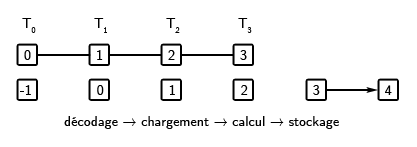
\includegraphics{images/misd.png}
        		\caption{Illustration d'une unité de traitement en
            \textit{pipelines}}
        		\label{fig:misd}
      	  \end{figure}
        \paragraph{MIMD} est la plus importante de nos jours. Exemples :
          \begin{itemize}
            \item multic\oe urs
            \item machines parallèles spécialisées HPC (\textit{Blue Gene})
            \item grappe (\textit{cluster}) : 10 à 1000 PC connectés via le
            réseau
            \item grille de calcul (grappes reparties dans le monde en plusieurs
            milles en distribué)
            \item CLOUD : service de calcul virtualisé à grande échelle
          \end{itemize}
      \subsubsection{Caractérisation}
        \paragraph{Mémoire partagée} Dans ce cas chaque processeur accède à la
        mémoire partagée en écrivant sur le bus (étranglement) et un autre
        processeur lit le mot écrit.
        \begin{figure}[!ht]
          \centering
          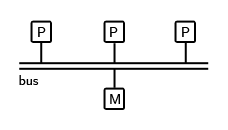
\includegraphics{images/shmem.png}
          \caption{\textit{Simetric Multi Processor}}
          \label{fig:smp}
        \end{figure}
        \begin{itemize}
          \item Les adresses sont les mêmes pour tous les processeurs.
          \item  Un seul accès est permis à la fois.
        \end{itemize}
        La mémoire partagée sert aux processeurs comme moyen de communication
        mais elle est plus lente que la fréquence des processeurs. On introduit
        alors l'architecture à cache (Core\texttrademark\ Duo, AMD DualCore avec
         L2 séparée):
        \begin{figure}[!ht]
         \centering
         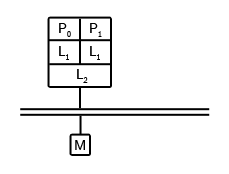
\includegraphics{images/shmc.png}
         \caption{\textit{Exemple d'architecture à cache}}
         \label{fig:shmc}
        \end{figure}
        \paragraph{Mémoire distribuée (voir la figure \ref{fig:mdistr})} En
        revanche en distribué chaque processeur a sa propre mémoire et la
        communication se fait par échange de messages via un réseau
        d'interconnexion (commutateur \textit{Myrinet} spécialisé, \textit{
        Gigabit Ethernet}, Internet ou NoC : \textit{Network on chip}). Les
        avantages de ce modèle sont l'indépendance des composantes, la
        modularité et la scalabilité de l'architecture.
        \begin{figure}[!ht]
          \centering
          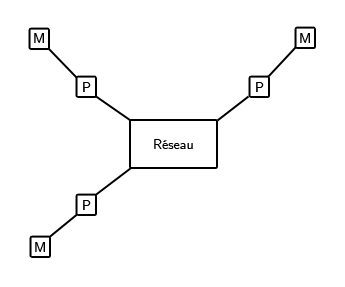
\includegraphics{images/mdistr.png}
          \caption{\textit{Modèle de mémoire distribuée}}
          \label{fig:mdistr}
        \end{figure}
    \subsection{Performance}
      Définitions :
      \begin{itemize}
        \item \textbf{accélération} (\textit{speed-up}) : \(S(n, p) =
        \frac{T_1(n)}{T_p(n)}\) où \(T_1(n)\) est le temps séquentiel d'un
        programme spécifique pour une donnée de taille \(n\) et \(T_p(n)\) le
        temps parallèle avec \(p\) processus
        \begin{itemize}
          \item si \(S < p\) alors il s'agit d'accélération sous-linéaire
          (normal)
          \item si \(S = p\) alors il s'agit d'accélération linéaire (rare)
          \item si \(S > p\) alors il s'agit d'accélération sur-linéaire
          (exceptionnel)
        \end{itemize}
        \item \textbf{éfficacité} : \(E(n, p) = \frac{S(n, p)}{p} =
        \frac{T_1(n)}{p \times T_p(n)}\)
        \item \textbf{coût total} : \(C(n, p) = p \times T_p(n)\)
      \end{itemize}
      \subsubsection{Loi d'Amdahl (1967)}
        Suppositions :
        \begin{itemize}
          \item \(T_1(n) = T_s(n) + T_p(n)\) où \(T_s(n)\) est la partie
          non-parallélisable et \(T_p(n)\) la partie parallélisable
          \item \(T_s(n) = f(n) \times T_1(n)\) où \(f(n)\) est la fraction
          séquentielle
          \item \(T_p(n) = (1 - f(n)) \times T_1(n)\)
        \end{itemize}
        Le meilleur temps parallèle possible est \(T_p(n) = T_s(n) +
        \frac{T_p(n)}{p} = (f(n) + \frac{1 - f(n)}{p}) \times T_1(n)\) d'où
        \(lim_{p\to\infty} S(n, p) = lim_{p\to\infty}\  \frac{1}{f(n) +
        \frac{1 - f(n)}{p}} = \frac{1}{f(n)}\). \\
        \indent \textit{Exemple :} \(\forall \ n,\ f(n) = 10\%\) donne
        l'accélération de 10 et l'éfficacité nulle.
    \subsection{Programmation}
      Étudions la technique de programmation parallèle sur un exemple :
      \paragraph{Évaluation d'un polynôme} \(P(x) = a + b \times x + c \times
      x^2 + d \times x ^ 3\) \\
      En séquentiel :
      \begin{lstlisting}
        for (i = 0; i < n; i++)
          res[i] = a + b * v[i] + c * v[i] ^ 2 + d * v[i] ^ 3;
      \end{lstlisting}
      En parallèle, on a trois possibilités :
      \begin{enumerate}
        \item \textbf{parallélisme des données} (s'assurer de l'indépendance des
         données) :
        \begin{lstlisting}
          parallel for (i = 0; i < (n - 1); i++)
            res[i] = P(v[i]);
        \end{lstlisting}
        Un compilateur parallèle produit un exécutable parallèle. Mais
        généralement le nombre de processeurs est inférieur à N. Comment
        répartir alors les itérations sur les processeurs ?
        \begin{enumerate}
          \item \textbf{distribution} cyclique : le processeur $r$ prend tous
          les $i$ avec $i\ \%\ p = r$
          \item \textbf{distribution par bloc} : $r \times \frac{N}{p} \leq i <
          (r + 1) \times \frac{N}{p}$
          \item \textbf{distribution par blocs cycliques} : pour $b$ une taille
          de blocs on a $\left \lfloor{\frac{i}{b}}\right \rfloor \%\ p = r$
        \end{enumerate}
        \item \textbf{parallélisme de tâches} (assurer la synchronisation) : $R
        = a + b \times v(i),\ S = c + d \times v(i),\ T = v(i) \times v(i),\
        res(i) = R + S \times T$. Néanmoins l'ordonnancement des systèmes de
        tâches est difficile.
        \item \textbf{parallélisme de flux} (\textit{pipelines}) : reformulation
         du calcul avec le schéma de Horner ressemble à $res(i) = a + v(i)
        \times (b + v(i) \times (c + v(i) \times d))$
        \begin{figure}[!ht]
          \centering
          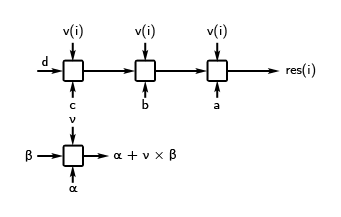
\includegraphics{images/pflux.png}
          \caption{\textit{Floating Point Multiply Add}}
          \label{fig:mdistr}
        \end{figure}
        \item \textbf{parallélisme de la mémoire vive} : implique un nombre
        arbitraire de processeurs synchronisés disposant des instruction
        habituelles (addition, multiplication, etc.) ainsi que l'utilisation
        d'une mémoire partagée. \\
        Dans ce cas on analyse deux types de ressources :
        \begin{itemize}
          \item le temps total d'une exécution
          \item le coût exprimé en nombre total d'instructions
        \end{itemize}
        \textit{\textbf{Exemple :} opération OU (algorithmes)} \\
        La donnée en entrée est un vecteur $a[]$ de base. La question qu'on se
        pose est de savoir s'il y a une seule valeur qui soit vraie. \\
        \begin{lstlisting}
          result = false;
          parallel for (i = 0; i < (n - 1); i++)
            if(a[i]) result = true;
          return result;
        \end{lstlisting}
        Le coût est de $O(n)$ et le temps est constant $O(1)$. \\
        Le problème est que plusieurs processeurs écrivent dans la même variable
        . On distingue alors \textit{Concurrent Read and Concurrent Write} dans
        la RAM parallèle ce qui n'est pas réaliste. Il faudrait donc mettre en
        place \textit{Concurrent Read and Exclusive Write} :
        \begin{lstlisting}
          parallel for (i = 0; i < (n - 1); i++)
            b[i] = a[i]; // tout acces est exclusif
          while (n > 1) {
            r = n % 2;
            m = floor(n / 2); // partie entiere inferieure
            n = m + r;
            parallel for (i = 0; i < (m - 1); i++)
              b[i] = (b[i] || b[i + n]);
          }
          return b[0];
        \end{lstlisting}
        Dans ce cas le temps est de $O(log(n))$ et le coût $O(n * log(n))$ le
        but étant d'avoir le coût de $O(n)$ avec $\frac{n}{log(n)}$ processeurs.
         \\
        Toujours est-il que l'accès concurrent à la mémoire est primordial. Il
        faut donc assurer la \textbf{cohérence} et la \textbf{performance}. \\
        \textit{\textbf{Exemple :}}
        \begin{lstlisting}
          tmp0 = a;
          tmp1 = a;
          tmp0 = tmp0 + 1;
          tmp1 = tmp1 + 1;
          a = tmp0;
          a = tmp1;
        \end{lstlisting}
        Ici la variable $a$ est augmentée deux fois : $2 \times op(a + 1)$ !
      \end{enumerate}
  \section{Communication MPI}
    \subsection{Instructions atomiques}
      Ce sont des instructions spécialisées caractérisées comme étant
      \textbf{indivisibles}, \textbf{linéarisables} et
      \textbf{non-interruptibles}. \\
      Pour déclarer une variable comme atomique on utilise la syntaxe suivante :
      \textit{unsigned \_Atomic int counter = 0} \\
      Ainsi toutes les opérations effectuées sur celle-ci sont atomiques et donc
      effectuées en une seule opération. Mais le coût en est énorme.
    \subsection{Passage de messages}
      Chaque acteur (processeur ou processus) dispose d'une adresse et d'un état
      séparés. Ils communiquent en mode \textit{peer-to-peer}. Ainsi on évite
      l'accès concurrent. \\
      Pour communiquer on utilise les fonctions \textit{send} (envoi de message)
       et \textit{recv} (réception de message). \\
      Plusieurs types de communication sont possibles :
      \begin{itemize}
        \item \textbf{fiable}
        \item \textbf{ordnonnée} (sans déséquencement)
        \item \textbf{synchrone} (aller-retours en direct)
        \item \textbf{asynchrone} (sans réponse instantannée)
        \item \textbf{bloquante}
      \end{itemize}
    \subsection{Autres primitives (macro communication)}
      \begin{enumerate}
        \item \textbf{synchronisation} [tous, pas de donnée] : attendre que tous les
        acteurs aient fini l'opération concernée pour pouvoir synchroniser
        \item \textbf{diffusion} (\textit{broadcast}) [1 à tous, le même
        message]
        \item \textbf{distribution} (\textit{scatter}) [1 à tous, $n$ messages
        différents]
        \item \textbf{rassemblement} (\textit{gather}) [tous à 1, $n$ messages
        différents]
        \item \textbf{commérage} (\textit{all-to-all}) [tous à tous, $n$
        messages différents]
        \item \textbf{transposition} (\textit{multiscatter}) [tous à tous, $n^2$
         messages différents]
        \item \textbf{réduction} : pour une opération $\otimes$ on a $d = \bigotimes_{i = 0}^{n - 1} d_i$
        \item \textbf{traduction} : diffusion
      \end{enumerate}
      Les six premières opérations sont inefficaces si elles sont réalisées en
      mode \textit{peer-to-peer}.
\end{document}
